\documentclass[12pt,a4paper]{article}

% --- Cấu hình Tiếng Việt và Font ---
\usepackage[utf8]{inputenc}
\usepackage[vietnamese]{babel}
\usepackage[T1]{fontenc}
\usepackage{times} % Font Times New Roman

% --- Định dạng lề và trình bày ---
\usepackage[left=3cm,right=2cm,top=2cm,bottom=2cm]{geometry}
\usepackage{indentfirst} % Thụt đầu dòng đoạn đầu
\usepackage{setspace}
\usepackage{float}
\onehalfspacing % Cách dòng 1.5

% --- Gói bổ trợ ---
\usepackage{amsmath, amssymb}
\usepackage{graphicx}
\usepackage{booktabs} % Bảng biểu chuyên nghiệp
\usepackage{multirow}
\usepackage{hyperref}
\usepackage{caption}
\usepackage{subcaption} % Chèn nhiều ảnh con
\usepackage{listings} % Chèn code nếu cần
\usepackage{xcolor}

\begin{document}

% --- PHẦN 2.3.2: PHÂN TÍCH THỐNG KÊ VĂN BẢN ---
\subsection{Phân tích thống kê văn bản (Text EDA)}

\subsubsection{Phân phối độ dài văn bản theo nhãn lớp}
Trước khi thực hiện tiền xử lý, tiến hành phân tích phân phối độ dài của các văn bản dựa trên số từ và số ký tự để hiểu rõ đặc trưng của tập dữ liệu giữa hai lớp Positive và Negative.

\begin{figure}[H]
    \centering
    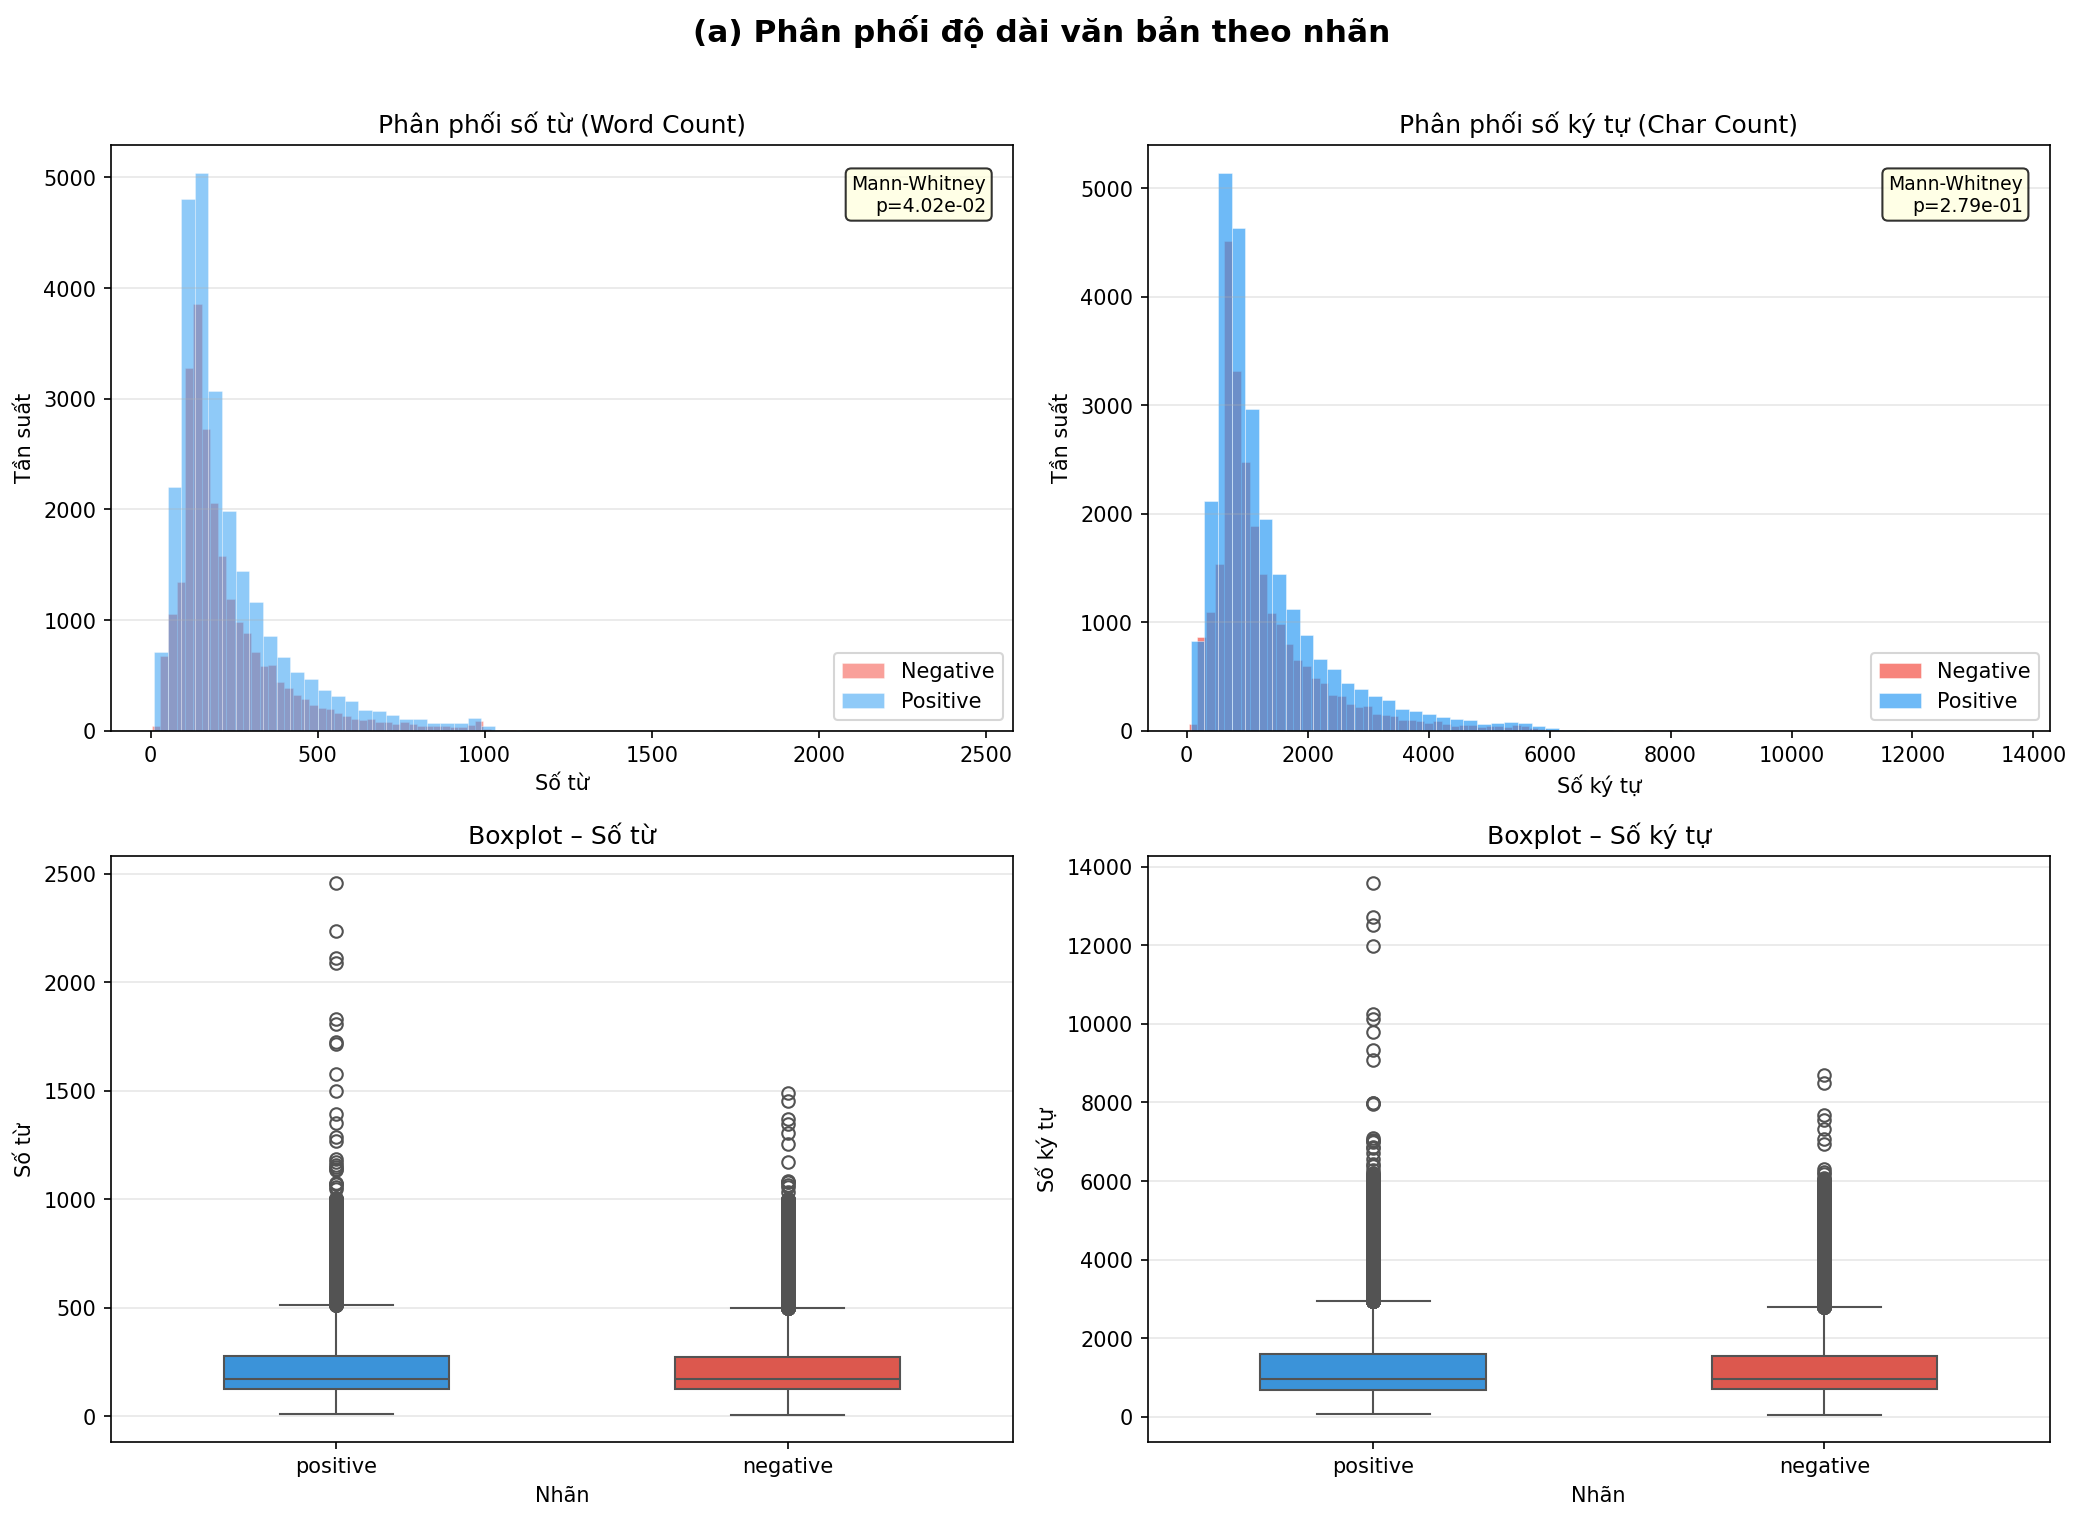
\includegraphics[width=0.9\textwidth]{eda_text/eda_a_length_distribution.png}
    \caption{Phân phối độ dài văn bản (số từ và số ký tự) theo nhãn lớp.}
    \label{fig:length_dist}
\end{figure}

\textbf{Kiểm định Mann-Whitney U:} 
Để xác định liệu có sự khác biệt đáng kể về mặt thống kê giữa độ dài của hai lớp hay không, sử dụng kiểm định phi tham số Mann-Whitney U trên cả hai tiêu chí:

\begin{itemize}
    \item \textbf{Độ dài theo số từ (Word count):} Kết quả thu được $p\text{-value} = 0.0402$. Vì $p < 0.05$, bác bỏ giả thuyết $H_0$, xác nhận rằng có sự khác biệt có ý nghĩa thống kê về độ dài tính theo số từ giữa hai lớp.
    \item \textbf{Độ dài theo số ký tự (Char count):} Kết quả thu được $p\text{-value} = 0.279$. Vì $p > 0.05$, không có đủ bằng chứng để bác bỏ giả thuyết $H_0$, cho thấy không có sự khác biệt đáng kể về độ dài tính theo số ký tự giữa hai lớp.
\end{itemize}

\textbf{Nhận xét:} Dựa trên kết quả kiểm định, hai lớp dữ liệu có xu hướng khác nhau về cách sử dụng số lượng từ ngữ trong một đánh giá, nhưng tổng số lượng ký tự trung bình lại có sự tương đồng đáng kể.

\subsubsection{Độ phong phú từ vựng và Word Cloud}
Sử dụng chỉ số \textbf{Type-Token Ratio (TTR)} để đo lường độ phong phú của từ vựng. Kết quả cho thấy cả hai lớp có độ đa dạng từ vựng tương đương nhau:
\begin{itemize}
    \item \textbf{Positive Class:} $TTR = 0.0313$ ($73,445$ types / $2,345,473$ tokens).
    \item \textbf{Negative Class:} $TTR = 0.0316$ ($70,633$ types / $2,234,420$ tokens).
\end{itemize}

Trực quan hóa Word Cloud cho lớp Positive và Negative.

\begin{figure}[H]
    \centering
    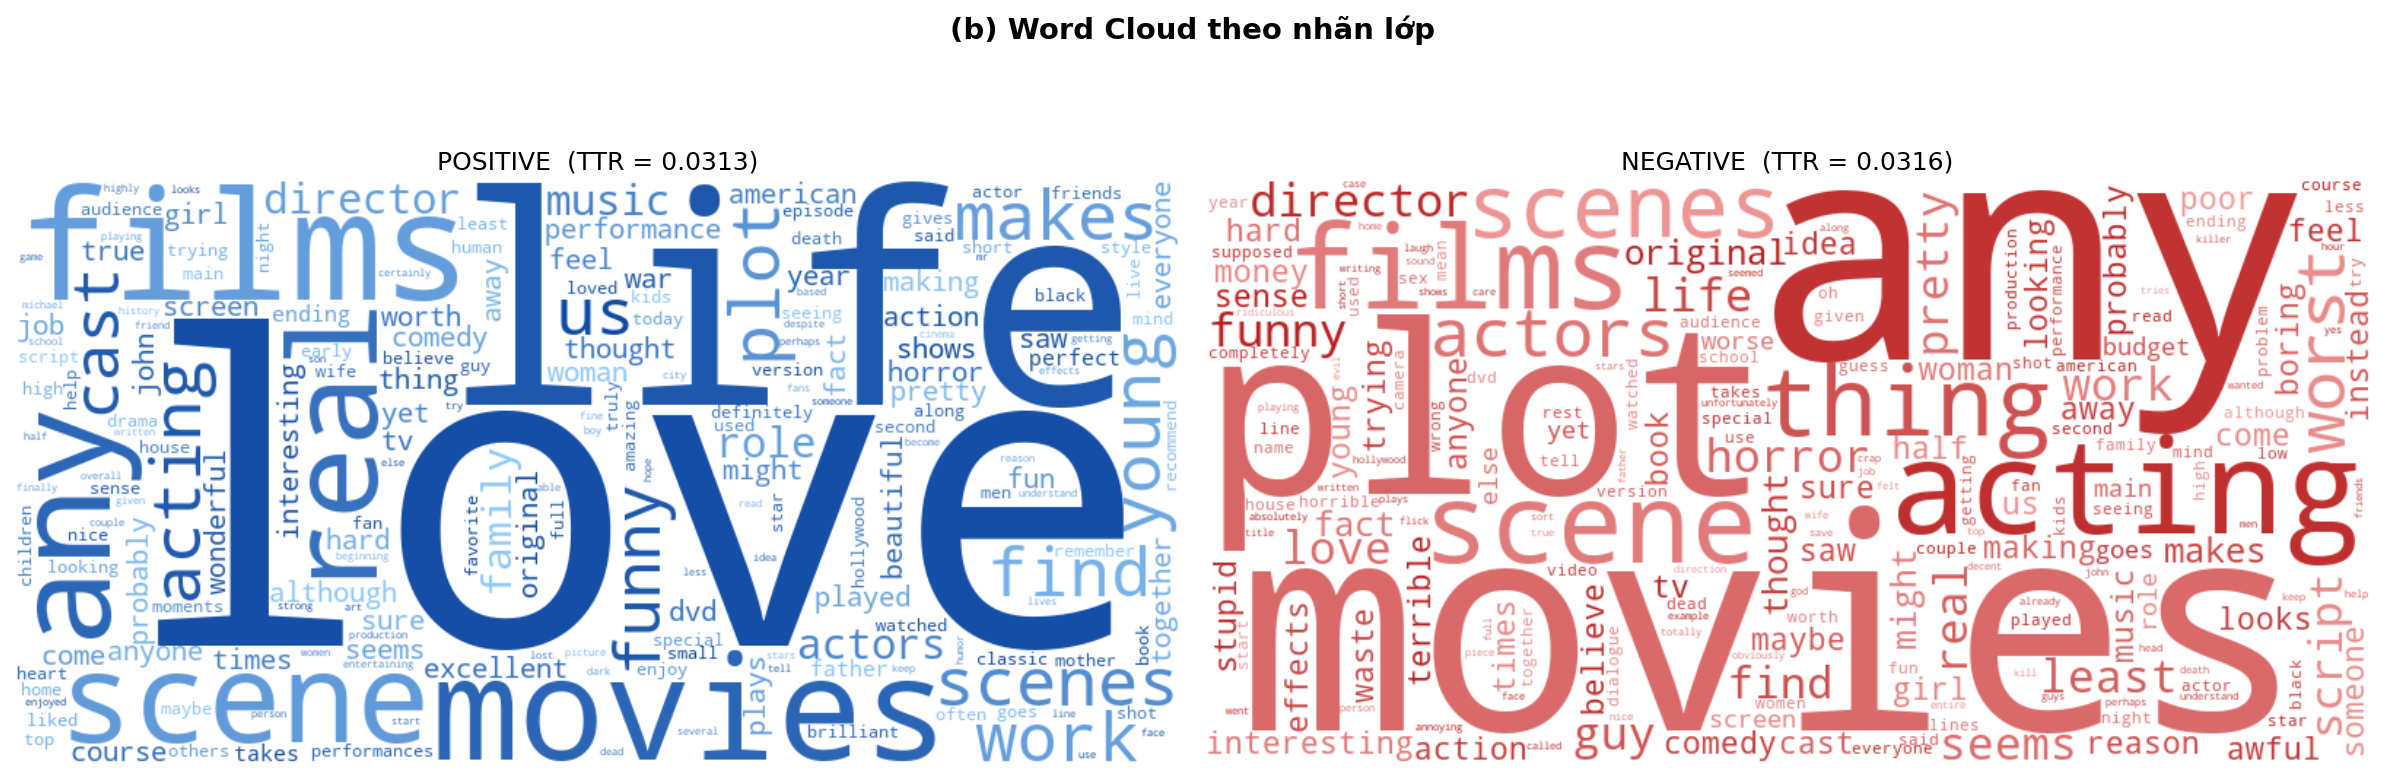
\includegraphics[width=0.9\textwidth]{eda_text/eda_b_wordcloud.png}
    \caption{Trực quan hóa Word Cloud cho lớp Positive và Negative.}
    \label{fig:wordcloud}
\end{figure}

Bảng \ref{tab:top_words} liệt kê danh sách 15 từ xuất hiện nhiều nhất trong mỗi lớp dữ liệu.

\begin{table}[H]
    \centering
    \caption{Thống kê Top 15 từ phổ biến nhất theo từng nhãn lớp.}
    \label{tab:top_words}
    \small
    \begin{tabular}{c|lc|lc}
        \toprule
        \textbf{STT} & \textbf{Từ (Positive)} & \textbf{Tần suất} & \textbf{Từ (Negative)} & \textbf{Tần suất} \\
        \midrule
        1  & love        & 8,692 & any      & 9,125 \\
        2  & life        & 8,137 & movies   & 8,313 \\
        3  & films       & 7,601 & plot     & 8,214 \\
        4  & movies      & 6,996 & acting   & 8,087 \\
        5  & any         & 5,919 & films    & 6,154 \\
        6  & scene       & 5,177 & scene    & 5,791 \\
        7  & real        & 5,115 & thing    & 5,782 \\
        8  & scenes      & 4,881 & scenes   & 5,601 \\
        9  & acting      & 4,780 & actors   & 4,971 \\
        10 & plot        & 4,773 & worst    & 4,888 \\
        11 & makes       & 4,700 & director & 4,812 \\
        12 & work        & 4,474 & life     & 4,780 \\
        13 & young       & 4,473 & funny    & 4,644 \\
        14 & find        & 4,467 & love     & 4,316 \\
        15 & us          & 4,340 & real     & 4,315 \\
        \bottomrule
    \end{tabular}
\end{table}


\subsubsection{Phân tích phân phối Zipf}
Thực hiện kiểm tra mức độ tuân theo định luật Zipf bằng cách vẽ biểu đồ log-log giữa tần suất và thứ hạng (rank) của các từ trong từ điển.

\begin{figure}[H]
    \centering
    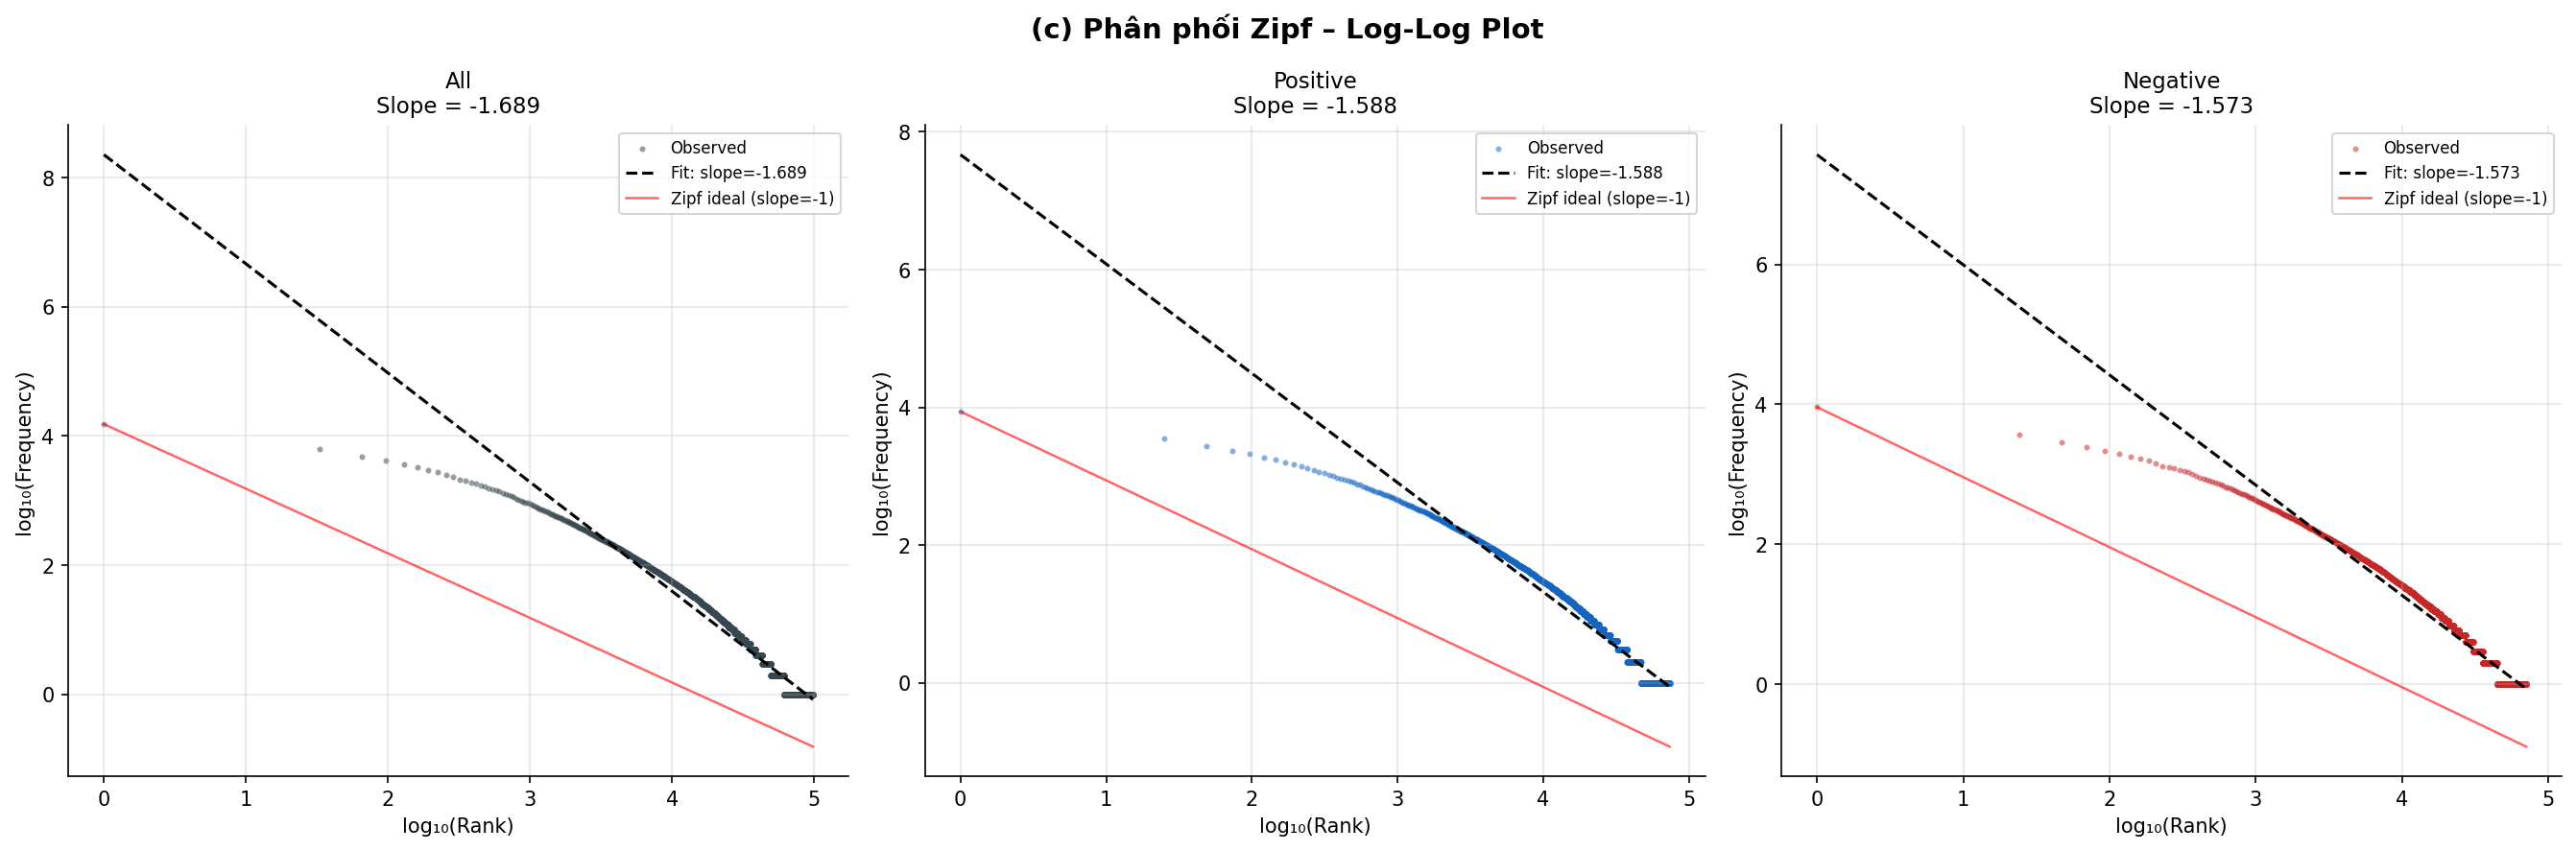
\includegraphics[width=0.9\textwidth]{eda_text/eda_c_zipf.png}
    \caption{Biểu đồ Log-Log thể hiện phân phối Zipf của tập dữ liệu.}
    \label{fig:zipf}
\end{figure}

\textbf{Nhận xét:} Dựa trên biểu đồ Hình \ref{fig:zipf}, đường phân phối của tập dữ liệu gần như song song với đường lý thuyết của định luật Zipf, cho thấy một số ít từ xuất hiện rất thường xuyên trong khi đại đa số các từ khác xuất hiện rất hiếm (long-tail distribution). Điều này khẳng định sự cần thiết của việc loại bỏ Stop words trong các bước tiếp theo.


% ==========================================
% PHẦN 2.3.3: CÁC KỸ THUẬT TIỀN XỬ LÝ VÀ PHÂN TÍCH TÁC ĐỘNG
% ==========================================
\subsection{Tiền xử lý dữ liệu}
% ==========================================
% PHẦN 2.3.3.a: PIPELINE CHUẨN HÓA VĂN BẢN
% ==========================================
\subsubsection{Pipeline chuẩn hóa văn bản}
Thực hiện xây dựng một quy trình chuẩn hóa văn bản (Preprocessing Pipeline) gồm 6 bước kế tiếp nhau nhằm loại bỏ nhiễu và làm sạch dữ liệu. Mục tiêu là giảm kích thước từ vựng (Vocabulary size) mà không làm mất đi các đặc trưng ngữ nghĩa quan trọng.

\begin{itemize}
    \item \textbf{Bước 1 - Lowercase:} Chuyển văn bản về chữ thường. 
    \item \textbf{Bước 2 - Remove HTML tags:} Loại bỏ các thẻ định dạng web như \texttt{<br />}.
    \item \textbf{Bước 3 \& 4 - Remove URLs, @Mentions, \#Hashtags:} Loại bỏ các liên kết và định danh mạng xã hội.
    \item \textbf{Bước 5 - Remove special chars:} Xóa bỏ các ký tự đặc biệt, chỉ giữ lại các dấu câu cơ bản. Đây là bước có tác động mạnh nhất đến dữ liệu.
    \item \textbf{Bước 6 - Normalize whitespace:} Loại bỏ các khoảng trắng thừa và ký tự điều khiển.
\end{itemize}

Để trực quan hóa sự thay đổi của dữ liệu, biểu đồ dưới đây so sánh phân phối độ dài văn bản của tập dữ liệu tại trạng thái gốc và sau khi đi qua toàn bộ Pipeline.

\begin{figure}[H]
    \centering
    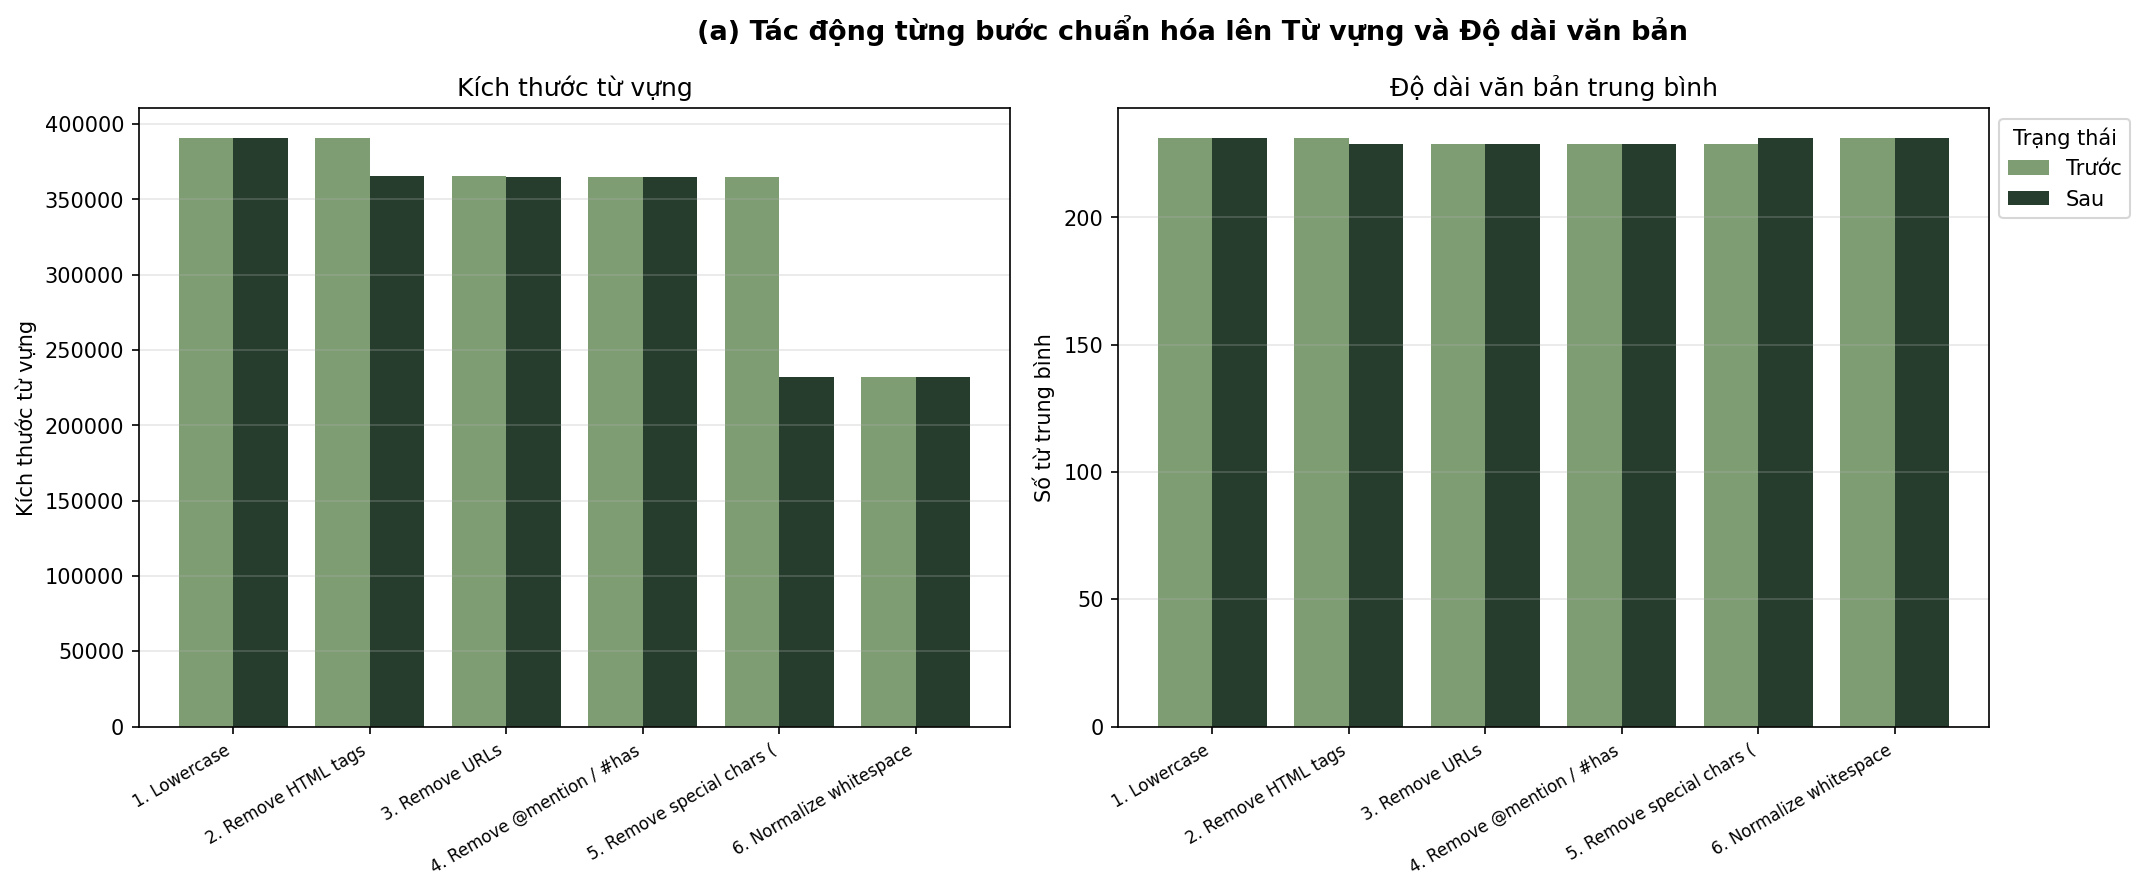
\includegraphics[width=0.9\textwidth]{preprocessing_text/a_preproc_a_pipeline_impact.png}
    \caption{Tác động của quá trình chuẩn hóa lên phân phối độ dài văn bản.}
    \label{fig:normalization_impact}
\end{figure}

Bảng \ref{tab:normalization_summary} chi tiết hóa sự biến động của kích thước từ vựng và độ dài văn bản qua từng bước xử lý cụ thể:

\begin{table}[H]
    \centering
    \caption{Thống kê chi tiết các bước trong Pipeline chuẩn hóa.}
    \label{tab:normalization_summary}
    \small
    \begin{tabular}{clcccc}
        \toprule
        \textbf{STT} & \textbf{Bước xử lý} & \textbf{Vocab sau} & \textbf{$\Delta$Vocab (\%)} & \textbf{AvgLen sau} & \textbf{$\Delta$AvgLen (\%)} \\
        \midrule
        1 & Lowercase & 390,931 & -0.00\% & 231.2 & -0.00\% \\
        2 & Remove HTML tags & 365,396 & -6.53\% & 228.9 & -0.99\% \\
        3 & Remove URLs & 365,226 & -0.05\% & 228.9 & -0.00\% \\
        4 & Remove @/\# tags & 365,103 & -0.03\% & 228.9 & -0.00\% \\
        5 & Remove special chars & 232,098 & -36.43\% & 231.3 & +1.08\% \\
        6 & Normalize whitespace & 232,098 & -0.00\% & 231.3 & -0.00\% \\
        \bottomrule
    \end{tabular}
\end{table}

\textbf{Phân tích kết quả:}
\begin{itemize}
    \item \textbf{Kích thước từ vựng:} Sau toàn bộ pipeline, kích thước từ vựng giảm mạnh từ \textbf{390,931} xuống còn \textbf{232,098} (giảm khoảng 40.6\%). Trong đó, bước loại bỏ ký tự đặc biệt (Bước 5) đóng góp mức giảm lớn nhất (36.43\%), cho thấy dữ liệu thô chứa rất nhiều ký tự nhiễu không mang giá trị phân loại.
    \item \textbf{Độ dài trung bình:} Chỉ số \texttt{AvgLen} biến động không đáng kể (dao động quanh mức 230 từ), chứng tỏ việc chuẩn hóa chủ yếu loại bỏ các token rác và gộp các biến thể từ vựng hơn là cắt bỏ nội dung chính của văn bản.
\end{itemize}

% ---------------- b -----------------
% ==========================================
% PHẦN 2.3.3.b: SO SÁNH CHIẾN LƯỢC TOKENIZATION
% ==========================================
\subsubsection{So sánh chiến lược Tokenization}
Thực hiện cài đặt và so sánh 4 chiến lược tách từ (Tokenization) khác nhau: Word-level (sử dụng thư viện NLTK và spaCy), Sentence-level, Subword-level (BPE thông qua thư viện \texttt{tokenizers} của HuggingFace) và Character-level. 

Mục tiêu là đánh giá sự cân bằng giữa kích thước từ vựng (Vocabulary size), tỉ lệ từ ngoài từ điển (OOV ratio) và độ dài chuỗi sau khi tách.

\begin{figure}[H]
    \centering
    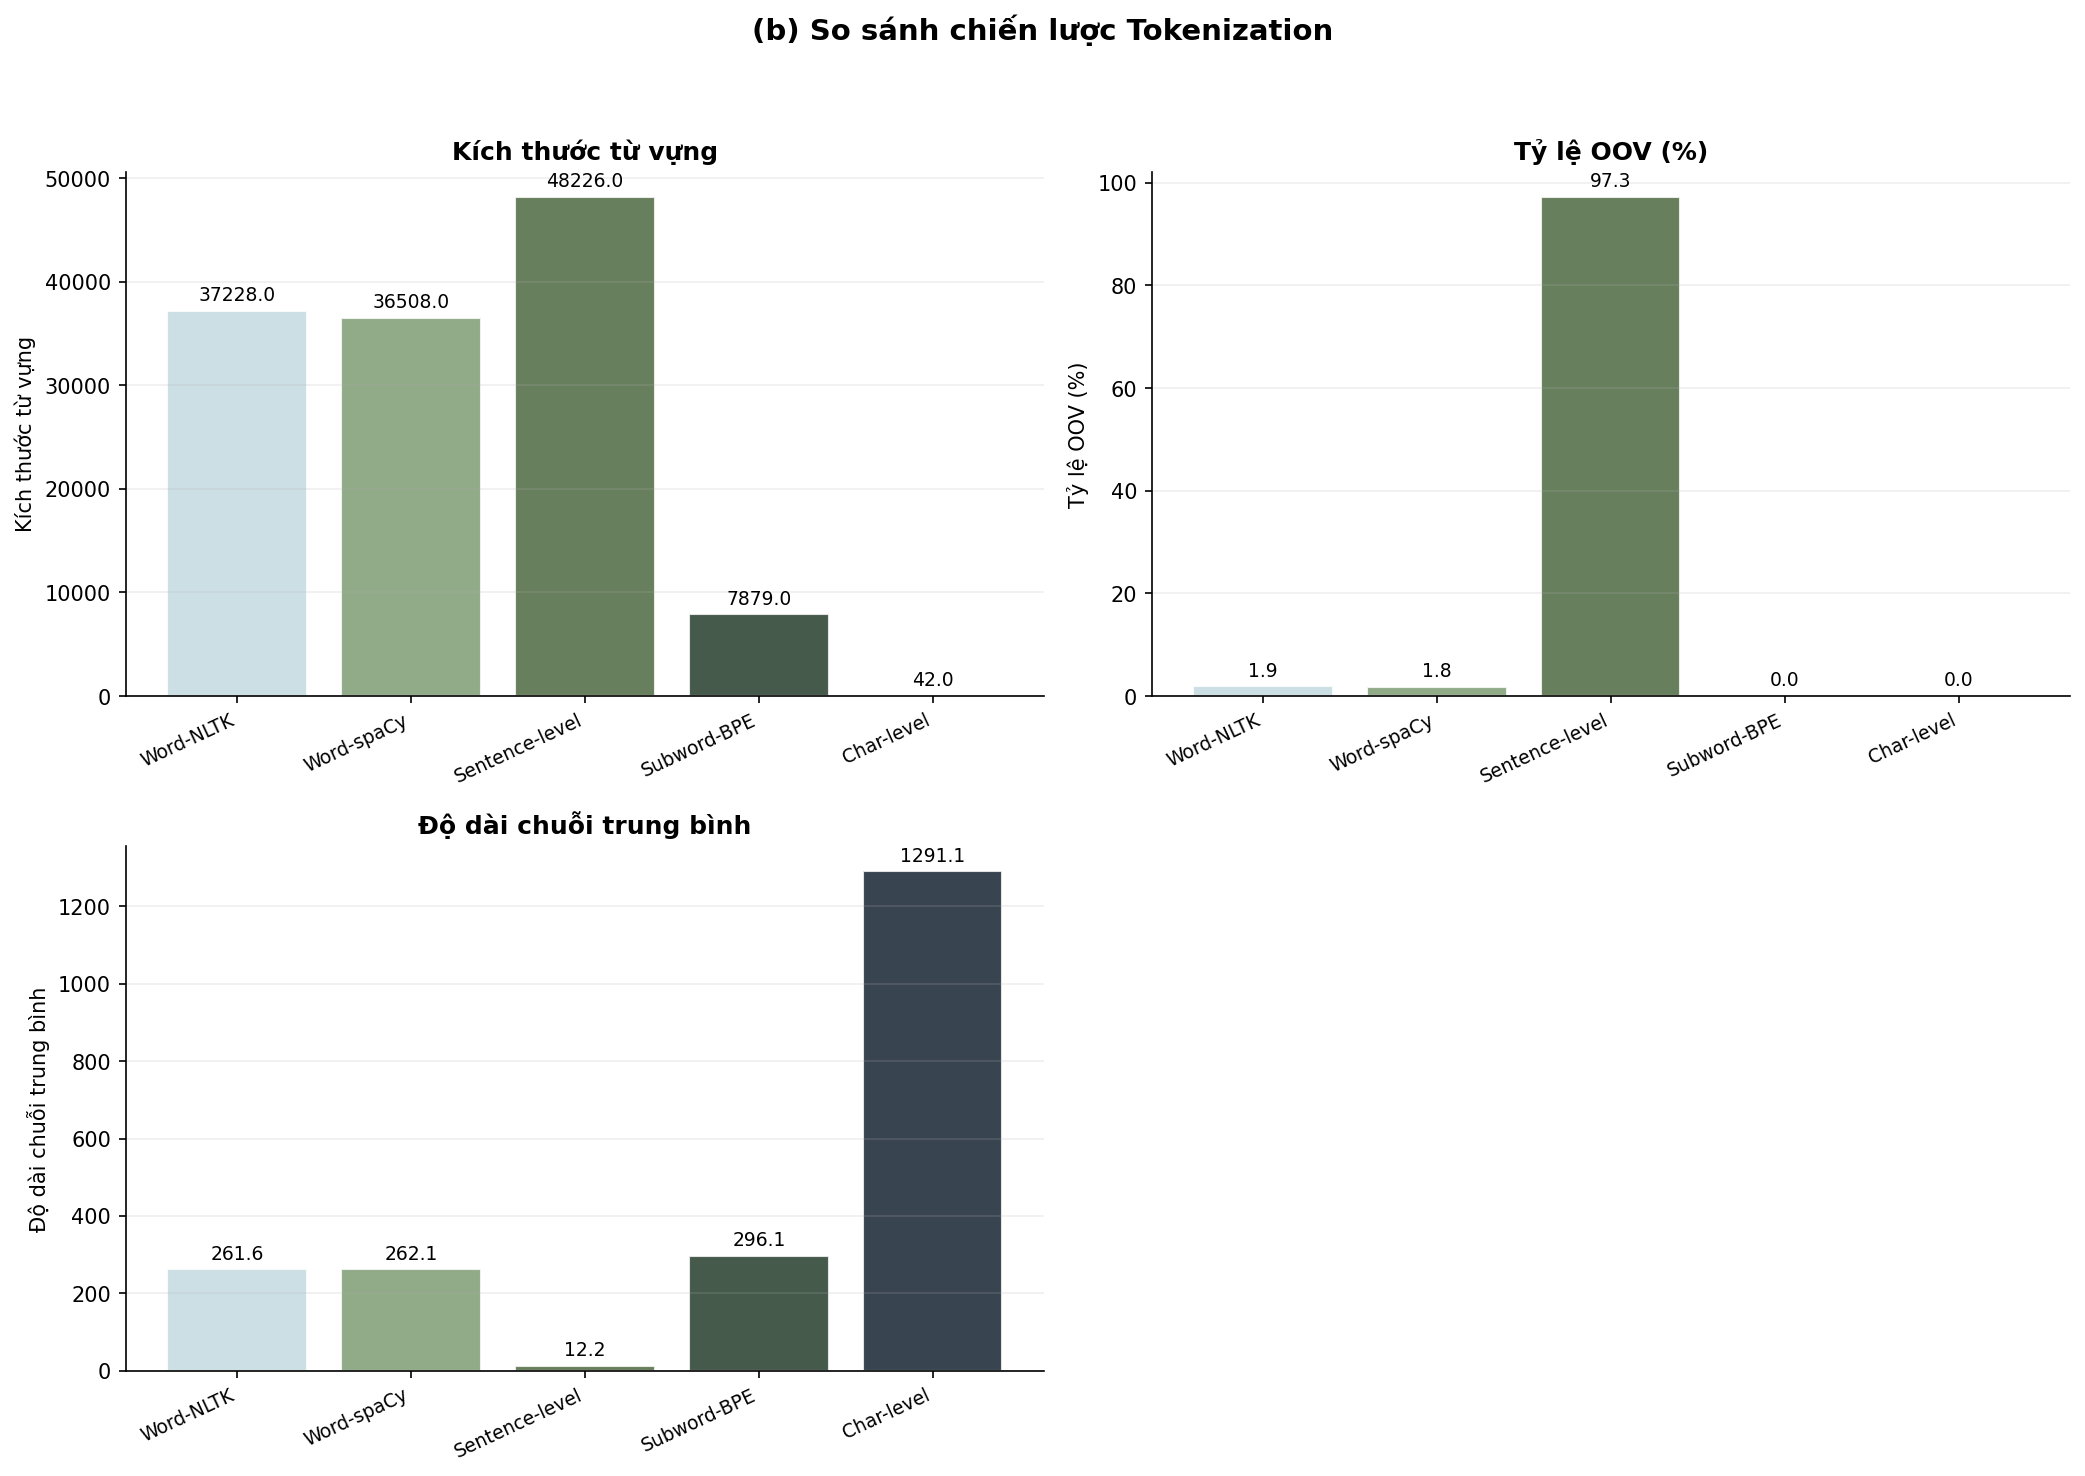
\includegraphics[width=0.9\textwidth]{preprocessing_text/b_tokenization.png}
    \caption{So sánh hiệu năng và đặc trưng giữa các chiến lược Tokenization.}
    \label{fig:tokenization_comparison}
\end{figure}

Bảng \ref{tab:tokenization_results} tổng hợp các chỉ số định lượng thu được từ thực nghiệm:

\begin{table}[H]
    \centering
    \caption{Kết quả so sánh các chiến lược Tokenization.}
    \label{tab:tokenization_results}
    \small
    \begin{tabular}{lccccc}
        \toprule
        \textbf{Chiến lược} & \textbf{Vocab size} & \textbf{OOV ratio (\%)} & \textbf{Avg seq len} & \textbf{Time (s/5k)} \\
        \midrule
        Word-NLTK & 37,228 & 1.885 & 261.6 & 13.61 \\
        Word-spaCy & 36,508 & 1.825 & 262.1 & 259.63 \\
        Sentence-level & 48,226 & 97.312 & 12.2 & 3.00 \\
        Subword-BPE & 7,879 & 0.004 & 296.1 & 13.15 \\
        Char-level & 42 & 0.000 & 1,291.1 & 0.00 \\
        \bottomrule
    \end{tabular}
\end{table}

\textbf{Phân tích và đánh giá:}
\begin{itemize}
    \item \textbf{Subword-BPE:} Đây là chiến lược tối ưu nhất khi chỉ với kích thước từ vựng rất nhỏ (7,879) nhưng đạt được tỉ lệ OOV gần như bằng 0 (0.004\%). Điều này giúp mô hình xử lý tốt các từ hiếm hoặc từ sai chính tả bằng cách chia nhỏ chúng thành các sub-units.
    \item \textbf{Word-level:} Cả NLTK và spaCy cho kết quả tương đồng về chất lượng. Tuy nhiên, spaCy tốn thời gian xử lý gấp gần 20 lần so với NLTK (259.63s so với 13.61s), cho thấy NLTK phù hợp hơn cho các tác vụ tiền xử lý nhanh trên tập dữ liệu lớn.
    \item \textbf{Sentence-level:} Có tỉ lệ OOV cực cao (97.312\%) do đơn vị tách quá lớn (cả câu), khiến việc bắt gặp lại chính xác một câu đã có trong từ điển là rất khó. Chiến lược này không hiệu quả cho bài toán phân loại văn bản đơn lẻ.
    \item \textbf{Character-level:} Loại bỏ hoàn toàn vấn đề OOV và có Vocab size nhỏ nhất (42), nhưng làm độ dài chuỗi tăng vọt (1,291.1 tokens), gây khó khăn cho việc huấn luyện các mô hình học sâu truyền thống do vấn đề phụ thuộc xa.
\end{itemize}

% ----------------------c---------------------------------
% ==========================================
% PHẦN 2.3.3.c: LOẠI BỎ STOP WORDS VÀ PHÂN TÍCH THÔNG TIN
% ==========================================
\subsubsection{Loại bỏ stop words và phân tích thông tin}
Stop words là các từ xuất hiện thường xuyên (như "the", "and", "is") nhưng thường mang ít giá trị ngữ nghĩa trong việc phân biệt cảm xúc. Thực hiện loại bỏ stop words và đánh giá tác động dựa trên chỉ số thông tin tương hỗ (Mutual Information - MI) và hiệu năng của mô hình Naive Bayes.

Để đảm bảo tính khách quan, kích thước từ vựng (Vocab size) được cố định ở mức 20,000 từ cho cả hai trường hợp.

\begin{figure}[H]
    \centering
    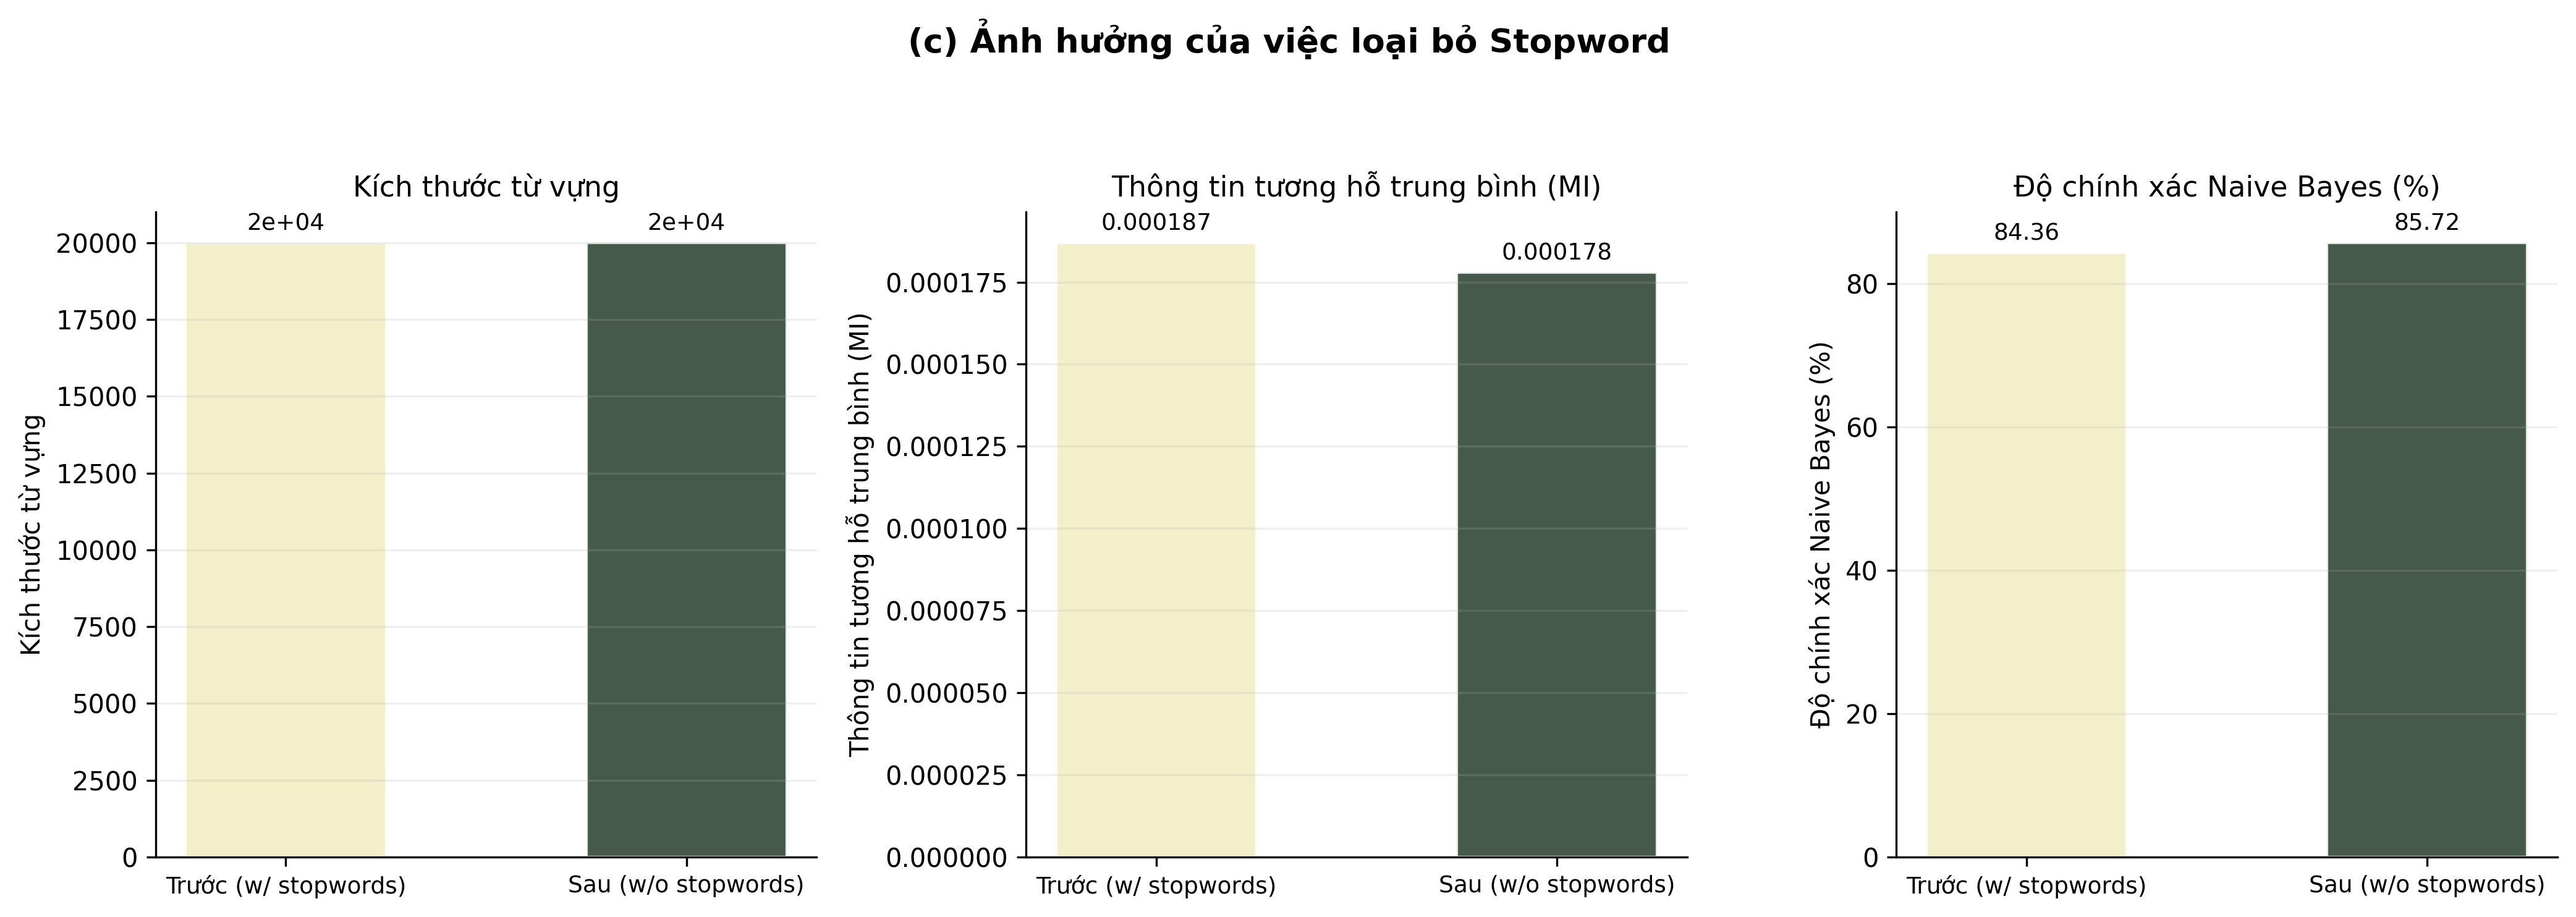
\includegraphics[width=0.9\textwidth]{preprocessing_text/c_stopwords.png}
    \caption{So sánh hiệu năng mô hình Naive Bayes trước và sau khi loại bỏ stop words.}
    \label{fig:stopwords_impact}
\end{figure}

Bảng \ref{tab:stopwords_comparison} thể hiện sự thay đổi về lượng tin và độ chính xác của mô hình:

\begin{table}[H]
    \centering
    \caption{Tác động của việc loại bỏ stop words đến MI và hiệu năng phân loại.}
    \label{tab:stopwords_comparison}
    \small
    \begin{tabular}{lcccc}
        \toprule
        \textbf{Trạng thái} & \textbf{Vocab size} & \textbf{Avg MI} & \textbf{NB CV Acc (\%)} & \textbf{NB Test Acc (\%)} \\
        \midrule
        Trước (w/ stopwords) & 20,000 & 0.000187 & 84.25 & 84.36 \\
        Sau (w/o stopwords) & 20,000 & 0.000178 & 85.42 & 85.72 \\
        \bottomrule
    \end{tabular}
\end{table}

\textbf{Thảo luận và nhận xét:}
\begin{itemize}
    \item \textbf{Về chỉ số MI:} Chỉ số Mutual Information trung bình giảm nhẹ từ $0.000187$ xuống $0.000178$. Điều này có thể giải thích là do một số stop words vẫn mang một lượng thông tin nhỏ về cấu trúc câu. Tuy nhiên, sự sụt giảm này là không đáng kể so với lợi ích về mặt tính toán.
    \item \textbf{Về hiệu năng:} Độ chính xác trên tập kiểm tra (Test Accuracy) tăng từ \textbf{84.36\%} lên \textbf{85.72\%}. Việc loại bỏ các từ phổ biến giúp mô hình Naive Bayes bớt bị "nhiễu" bởi các từ xuất hiện dày đặc ở cả hai lớp, từ đó tập trung tốt hơn vào các từ mang tính biểu cảm mạnh (sentiment-bearing words).
    \item \textbf{Kết luận:} Việc loại bỏ stop words không phải lúc nào cũng làm tăng MI nhưng trong bài toán phân loại cảm xúc phim này, nó rõ ràng giúp cải thiện hiệu năng và giảm độ phức tạp của không gian đặc trưng.
\end{itemize}
%------------------------d--------------------------------
\subsubsection{Stemming, Lemmatization và so sánh định lượng}
Tiến hành cài đặt và so sánh ba kỹ thuật biến đổi gốc từ phổ biến: \textbf{Porter Stemmer}, \textbf{Snowball Stemmer} và \textbf{WordNet Lemmatizer}. Mục tiêu là đưa các biến thể của từ về cùng một dạng gốc nhằm giảm số lượng đặc trưng và xử lý sự đồng nghĩa về mặt hình thái.

Để đánh giá chất lượng, sử dụng hai chỉ số:
\begin{itemize}
    \item \textbf{Collision rate (Tỉ lệ va chạm):} Tỉ lệ các từ khác nhau bị ánh xạ về cùng một chuỗi gốc (giá trị càng cao cho thấy mức độ gộp từ càng mạnh).
    \item \textbf{CV Accuracy (\%):} Độ chính xác trung bình khi thực hiện kiểm tra chéo (Cross-validation) với mô hình Logistic Regression.
\end{itemize}

\begin{figure}[H]
    \centering
    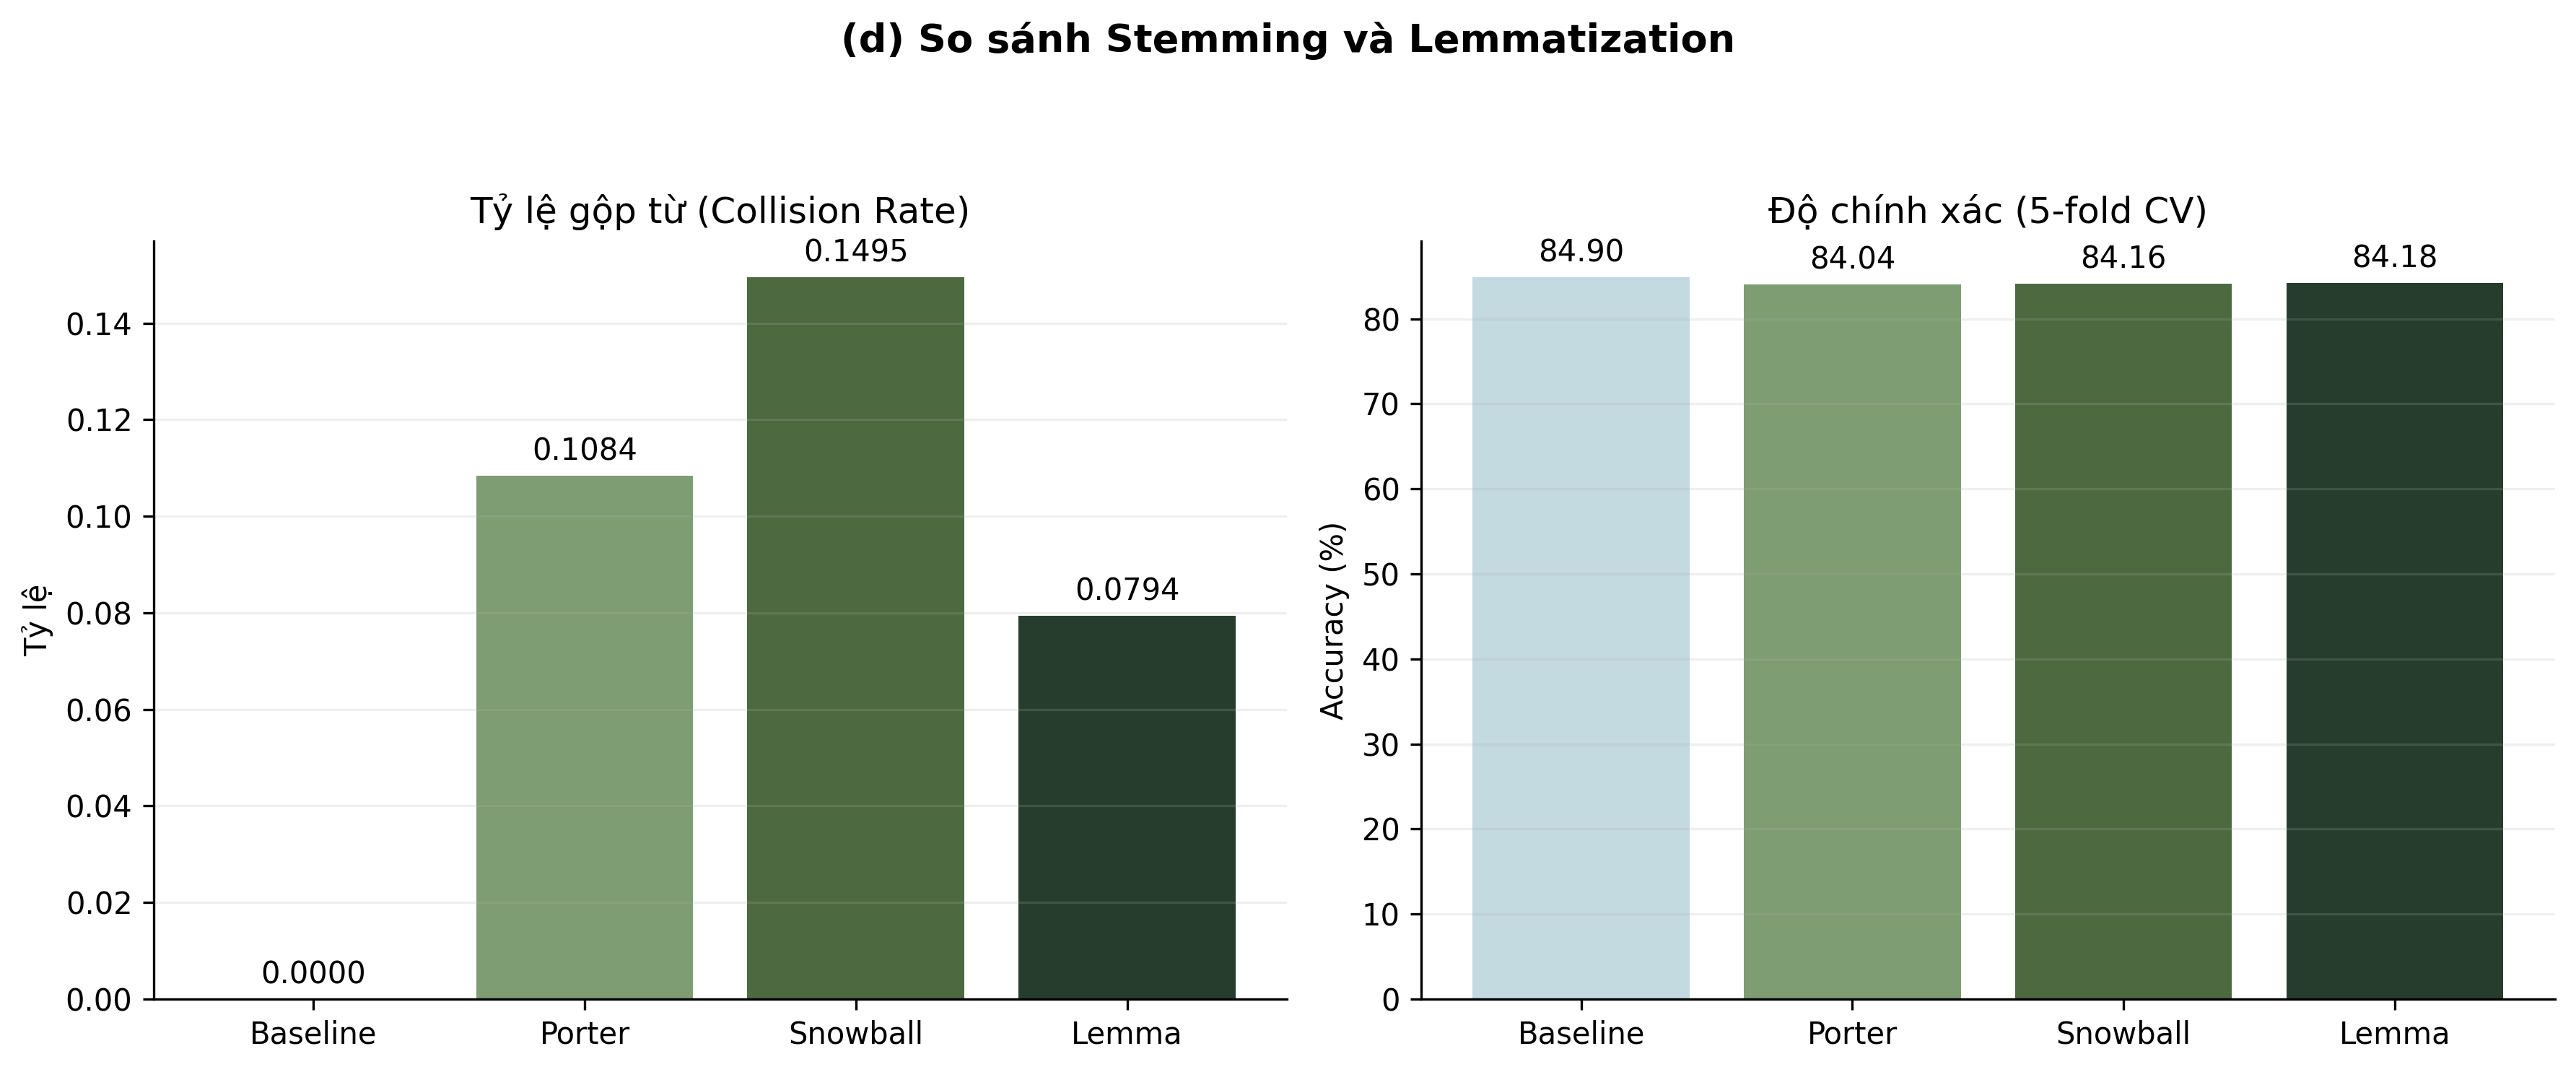
\includegraphics[width=0.9\textwidth]{preprocessing_text/d_stemming_comparison.png}
    \caption{So sánh tác động của Stemming và Lemmatization đến hiệu năng mô hình.}
    \label{fig:stem_lem_impact}
\end{figure}

Bảng \ref{tab:stem_lem_results} tổng hợp kết quả định lượng thu được:

\begin{table}[H]
    \centering
    \caption{So sánh hiệu năng giữa các phương pháp biến đổi gốc từ.}
    \label{tab:stem_lem_results}
    \small
    \begin{tabular}{lcc}
        \toprule
        \textbf{Phương pháp} & \textbf{Collision rate} & \textbf{CV Accuracy (\%)} \\
        \midrule
        Baseline (Không xử lý) & 0.0000 & \textbf{84.90} \\
        Porter Stemmer         & 0.1084 & 84.04 \\
        Snowball Stemmer       & 0.1495 & 84.16 \\
        WordNet Lemmatizer     & \textbf{0.0794} & 84.18 \\
        \bottomrule
    \end{tabular}
\end{table}

\textbf{Phân tích kết quả:}
\begin{itemize}
    \item \textbf{Về tỉ lệ va chạm (Collision rate):} \textbf{Snowball Stemmer} có tỉ lệ va chạm cao nhất (0.1495), cho thấy nó thực hiện cắt tỉa từ ngữ mạnh tay hơn so với Porter. Ngược lại, \textbf{Lemmatizer} có tỉ lệ va chạm thấp nhất (0.0794) vì nó dựa trên từ điển và ngữ pháp để tìm dạng gốc chuẩn (lemma), thay vì chỉ cắt bỏ hậu tố một cách máy móc.
    \item \textbf{Về độ chính xác:} Một quan sát đáng chú ý là \textbf{Baseline} đạt độ chính xác cao nhất (84.90\%). Việc áp dụng Stemming hay Lemmatization trong trường hợp này làm giảm nhẹ hiệu năng mô hình (xuống mức khoảng 84.0\% - 84.2\%). 
    \item \textbf{Thảo luận:} Kết quả này cho thấy đối với tập dữ liệu đánh giá phim, việc giữ nguyên các biến thể của từ (ví dụ: "acting", "acts", "acted") có thể cung cấp nhiều thông tin về sắc thái biểu cảm hơn là gộp chúng lại. Trong ba phương pháp xử lý, \textbf{Lemmatizer} cho kết quả tốt nhất nhờ giữ được tính trọn vẹn của từ vựng cao nhất.
\end{itemize}
%-------------------------e----------------------------------
% ==========================================
% PHẦN 2.3.3.e: VECTOR HÓA VĂN BẢN VÀ PHÂN TÍCH KHÔNG GIAN ĐẶC TRƯNG
% ==========================================
\subsubsection{Vector hóa văn bản và phân tích không gian đặc trưng}
Thực hiện biểu diễn văn bản dưới ba dạng vector hóa khác nhau: \textbf{Bag-of-Words (BoW)}, \textbf{TF-IDF (ngram với $n \in \{1, 2, 3\}$)} và \textbf{Word2Vec} (huấn luyện trên tập dữ liệu thực tế). Mục tiêu là đánh giá khả năng biểu diễn thông tin của từng phương pháp thông qua độ thưa (Sparsity), độ tương đồng (Cosine Similarity) và khả năng tách lớp.

\begin{figure}[H]
    \centering
    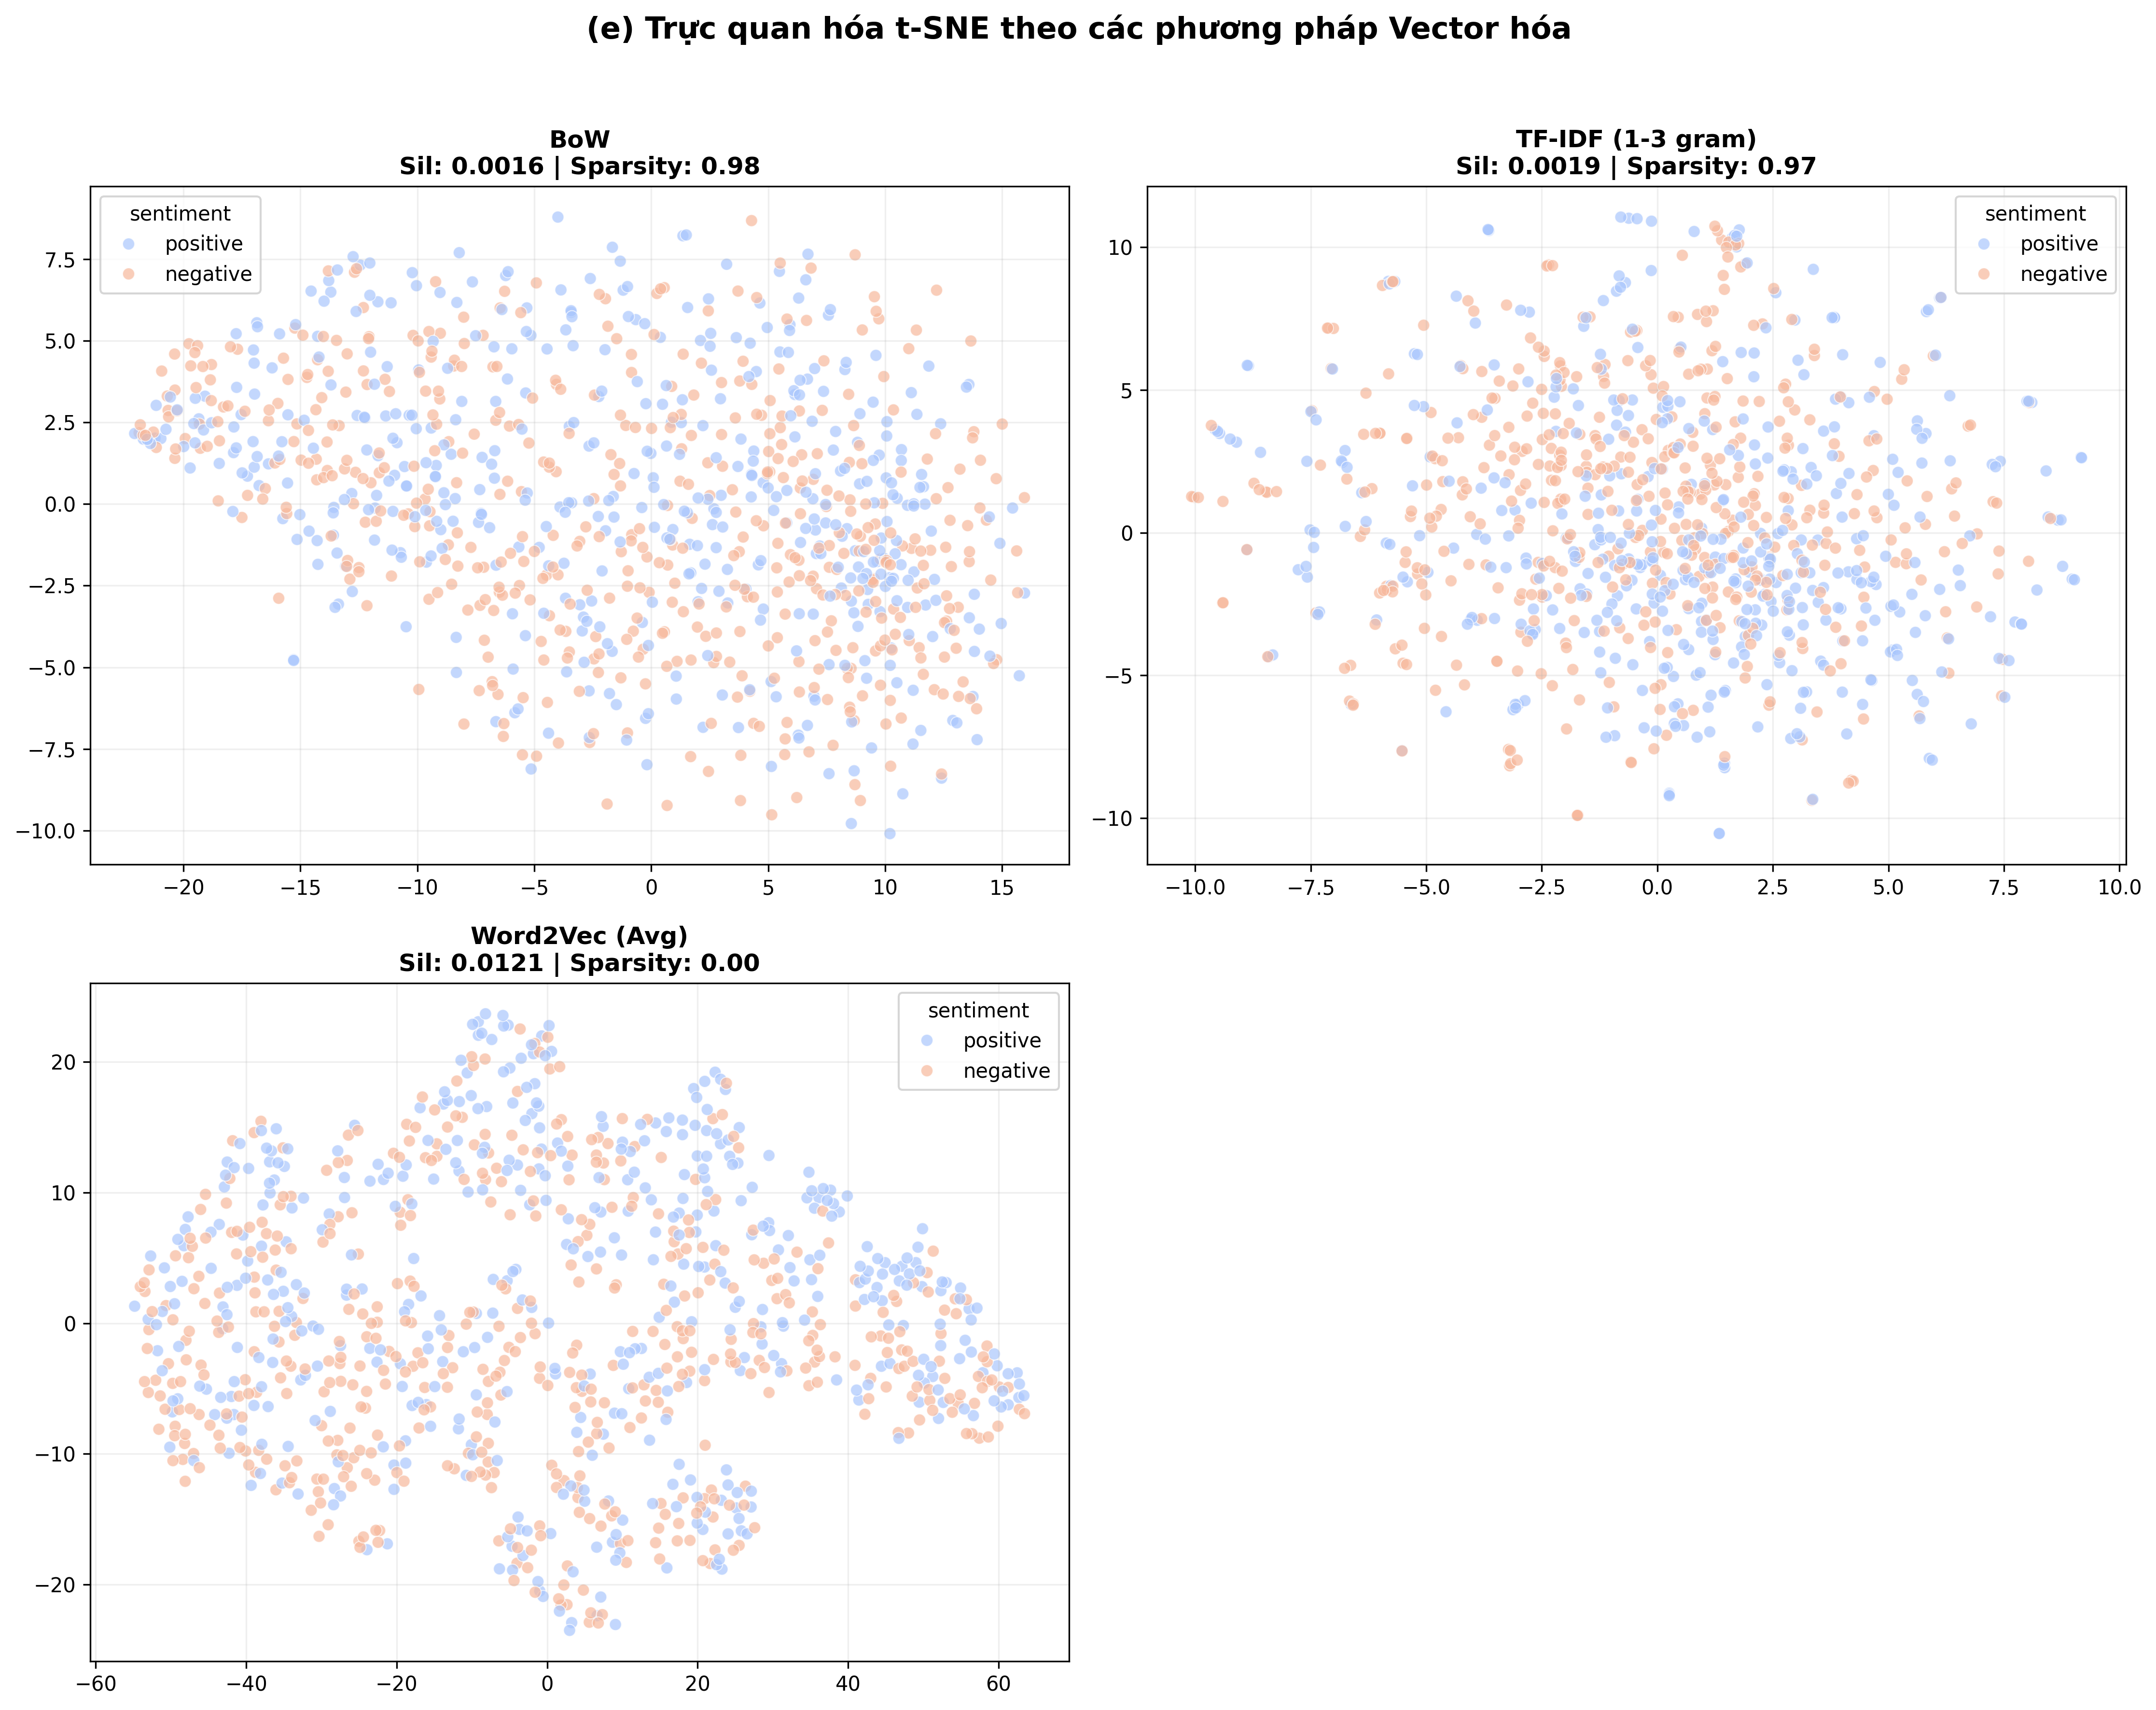
\includegraphics[width=0.9\textwidth]{preprocessing_text/e_vectorization_comparison.png}
    \caption{Trực quan hóa t-SNE 2D của các phương pháp vector hóa.}
    \label{fig:tsne_vectorization}
\end{figure}

Bảng \ref{tab:vectorization_results} tổng hợp các thông số đặc trưng của không gian đặc trưng:

\begin{table}[H]
    \centering
    \caption{So sánh các phương pháp biểu diễn văn bản.}
    \label{tab:vectorization_results}
    \small
    \begin{tabular}{lccccc}
        \toprule
        \textbf{Phương pháp} & \textbf{Số chiều} & \textbf{Độ thưa} & \textbf{Intra-Sim} & \textbf{Inter-Sim} & \textbf{Silhouette} \\
        \midrule
        BoW & 5,000 & 0.9761 & 0.5343 & 0.5289 & 0.0016 \\
        TF-IDF (1-3 gram) & 5,000 & 0.9663 & 0.1388 & 0.1353 & 0.0019 \\
        Word2Vec (Avg) & 100 & \textbf{0.0000} & 0.9981 & 0.9981 & \textbf{0.0121} \\
        \bottomrule
    \end{tabular}
\end{table}

\textbf{Phân tích kết quả:}
\begin{itemize}
    \item \textbf{Độ thưa (Sparsity):} BoW và TF-IDF tạo ra các ma trận cực kỳ thưa (lần lượt là 97.61\% và 96.63\%), điều này gây khó khăn về mặt lưu trữ và tính toán khi tập dữ liệu mở rộng. Ngược lại, \textbf{Word2Vec} cung cấp các vector dày đặc (dense) với số chiều thấp (100) nhưng chứa đựng nhiều thông tin nén.
    \item \textbf{Độ tương đồng (Intra vs Inter Similarity):} 
    \begin{itemize}
        \item Đối với BoW và TF-IDF, độ tương đồng nội lớp (Intra-Sim) chỉ nhỉnh hơn độ tương đồng liên lớp (Inter-Sim) một khoảng rất nhỏ.
        \item Word2Vec cho chỉ số tương đồng rất cao ($\approx 0.9981$), cho thấy các vector trong không gian nhúng nằm rất sát nhau.
    \end{itemize}
    \item \textbf{Khả năng tách lớp:} Chỉ số \textbf{Silhouette Score} của Word2Vec (0.0121) cao vượt trội so với BoW và TF-IDF. Điều này chứng tỏ rằng mặc dù không gian nhúng dày đặc, Word2Vec vẫn tạo ra các cụm dữ liệu có cấu trúc tách biệt tốt hơn về mặt ngữ nghĩa so với phương pháp dựa trên tần suất từ đơn thuần.
\end{itemize}
%-----------------------f-----------------------------
% ==========================================
% PHẦN 2.3.3.f: BIỂU DIỄN NGỮ NGHĨA BẰNG SENTENCE TRANSFORMER
% ==========================================
\subsubsection{[Nâng cao] Biểu diễn ngữ nghĩa bằng Sentence Transformer}
Trong phần này, Tiến hành thực nghiệm với mô hình tiền huấn luyện (pretrained) \texttt{all-MiniLM-L6-v2} từ thư viện \texttt{sentence-transformers}. Khác với TF-IDF chỉ dựa trên tần suất từ, mô hình này sử dụng cơ chế Attention để tạo ra các embedding đại diện cho ý nghĩa toàn văn bản trong không gian đa chiều.

Thực hiện so sánh chất lượng phân cụm thông qua thuật toán K-Means (Silhouette score) và hiệu năng phân loại bằng mô hình Linear SVM.

\begin{figure}[H]
    \centering
    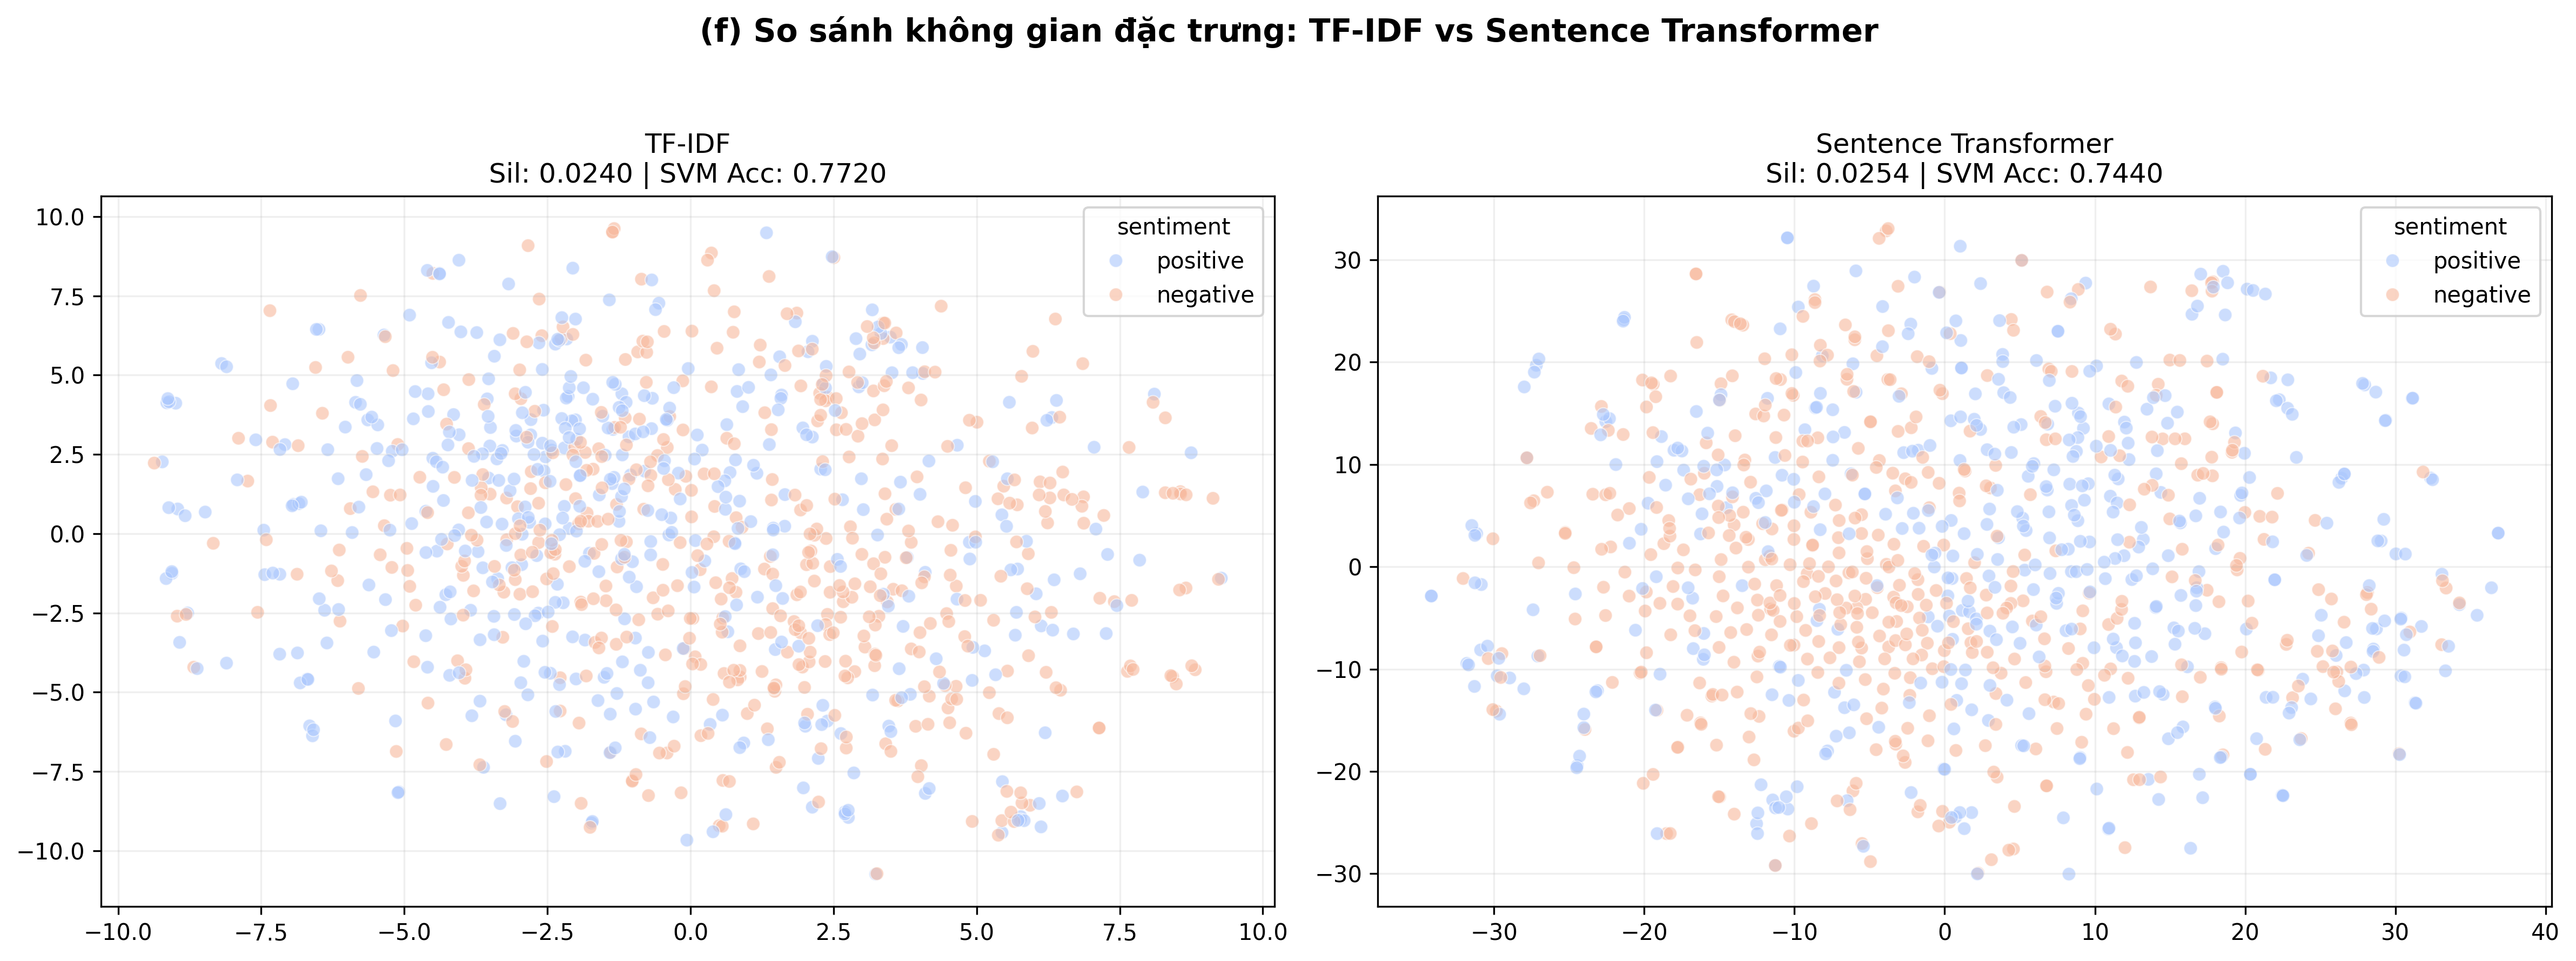
\includegraphics[width=0.9\textwidth]{preprocessing_text/f_semantic_comparison_viz.png}
    \caption{So sánh không gian đặc trưng giữa TF-IDF và Sentence Transformer.}
    \label{fig:transformer_vs_tfidf}
\end{figure}

Bảng \ref{tab:transformer_results} trình bày kết quả so sánh định lượng:

\begin{table}[H]
    \centering
    \caption{So sánh TF-IDF và Sentence Transformer embeddings.}
    \label{tab:transformer_results}
    \small
    \begin{tabular}{lcc}
        \toprule
        \textbf{Phương pháp} & \textbf{Silhouette Score} & \textbf{SVM Accuracy} \\
        \midrule
        TF-IDF & 0.0240 & \textbf{0.7720} \\
        Sentence Transformer & \textbf{0.0254} & 0.7440 \\
        \bottomrule
    \end{tabular}
\end{table}

\textbf{Giải thích và Thảo luận:}
\begin{itemize}
    \item \textbf{Về chất lượng biểu diễn (Silhouette):} Sentence Transformer đạt chỉ số Silhouette cao hơn (0.0254 so với 0.0240). Điều này khẳng định khả năng biểu diễn ngữ nghĩa vượt trội của mô hình Transformer; các văn bản có cùng ý nghĩa (ví dụ: "good movie" và "great film") được đưa về gần nhau hơn trong không gian vector dù không dùng chung từ khóa.
    \item \textbf{Về hiệu năng phân loại (Accuracy):} Đáng chú ý là TF-IDF lại cho độ chính xác cao hơn (77.2\% so với 74.4\%). Điều này có thể được giải thích do:
    \begin{enumerate}
        \item \textbf{Đặc trưng tập dữ liệu:} Trong các bài toán Sentiment Analysis đơn giản, các từ khóa cực đoan (như "worst", "excellent") đóng vai trò quyết định. TF-IDF làm nổi bật các từ này rất hiệu quả.
        \item \textbf{Fine-tuning:} Mô hình Sentence Transformer đang được sử dụng ở dạng "off-the-shelf" (chưa được tinh chỉnh trên tập dữ liệu chuyên biệt về phim), dẫn đến việc các vector đặc trưng có thể chưa hoàn toàn tối ưu cho nhãn lớp cụ thể của bài toán.
    \end{enumerate}
\end{itemize}

\textbf{Kết luận:} TF-IDF vẫn là một baseline rất mạnh cho các bài toán phân loại văn bản dựa trên từ khóa. Tuy nhiên, Sentence Transformer mang lại không gian đặc trưng giàu ngữ nghĩa hơn, có tiềm năng phát triển tốt hơn nếu được thực hiện Fine-tuning hoặc áp dụng cho các tác vụ tìm kiếm tương đồng ngữ nghĩa.









\end{document}